\documentclass{article}   
\usepackage[left=1.5cm,right=1.5cm,top=2.3cm,bottom=2.3cm]{geometry}		
\usepackage[utf8]{inputenc} 										
%\usepackage[french]{babel}
\usepackage{fancyhdr}								
\usepackage{hyperref}								
\usepackage{booktabs,multirow,hhline}		
\usepackage{graphicx}				
\usepackage{bibentry}
\usepackage{wrapfig,caption}
\usepackage{subcaption}
\usepackage[compact]{titlesec}
\titlespacing{\section}{0pt}{2ex}{1ex}
\titlespacing{\subsection}{0pt}{1ex}{0ex}
\titlespacing{\subsubsection}{0pt}{0.5ex}{0ex}
\usepackage{color}												
\usepackage[dvipsnames]{xcolor}								
\usepackage{amsmath,amssymb,amsthm,nicefrac}
\usepackage{mathrsfs}										
\usepackage{wasysym,marvosym}
\usepackage{mathtools}
\usepackage{verbatim}										
\usepackage{minted}										
\usepackage{lipsum}
\usepackage{tikz}
\usepackage[american]{circuitikz}
\usepackage{siunitx}
\usepackage{physics}
\usepackage{float}
\usepackage{movie15}
\usepackage{multicol}

\usepackage[backend=biber, style=numeric]{biblatex}
\addbibresource{references.bib} %Imports bibliography file


\parindent=0pt									
\parskip=6pt									

\fancyheadoffset{0 cm}	

%---------------
\begin{document}

\begin{center}

    {\Large \textbf{Functional gradients in geometrically embedded networks}}\\
    
    \vspace{10 pt}
    Antoine Légaré,$^{1}$ \\
    \vspace{5 pt}
    
    $^1$\textit{Département de biochimie, de microbiologie et de bio-informatique, Université Laval, Québec (Québec), Canada}\\
    

\end{center}

\vspace{4 pt}

Lorem ipsum lorem ipsum. Lorem ipsum lorem ipsum. Lorem ipsum lorem ipsum. Lorem ipsum lorem ipsum. Lorem ipsum lorem ipsum. Lorem ipsum lorem ipsum. Lorem ipsum lorem ipsum. Lorem ipsum lorem ipsum. Lorem ipsum lorem ipsum. Lorem ipsum lorem ipsum. Lorem ipsum lorem ipsum. Lorem ipsum lorem ipsum. Lorem ipsum lorem ipsum. Lorem ipsum lorem ipsum. Lorem ipsum lorem ipsum. Lorem ipsum lorem ipsum. Lorem ipsum lorem ipsum. Lorem ipsum lorem ipsum. Lorem ipsum lorem ipsum. Lorem ipsum lorem ipsum. Lorem ipsum lorem ipsum. Lorem ipsum lorem ipsum. Lorem ipsum lorem ipsum. Lorem ipsum lorem ipsum. Lorem ipsum lorem ipsum. Lorem ipsum lorem ipsum. Lorem ipsum lorem ipsum. Lorem ipsum lorem ipsum. Lorem ipsum lorem ipsum. Lorem ipsum lorem ipsum. Lorem ipsum lorem ipsum. Lorem ipsum lorem ipsum.

\vspace{10 pt}

\begin{multicols}{2}

\section*{Introduction}

\section*{Results}

\subsection*{Functional and geometric correspondence emerges in locally connected neural networks}

\subsection*{Long-distance connections constrain geometric mode wavelengths}

\subsection*{The emergence of geometric modes is independent of volume shape or dynamics}

\subsection*{Geometric modes in physical networks}

\subsection*{Analytic results and stuff}

\begin{figure*}[t!]
    \centering
%    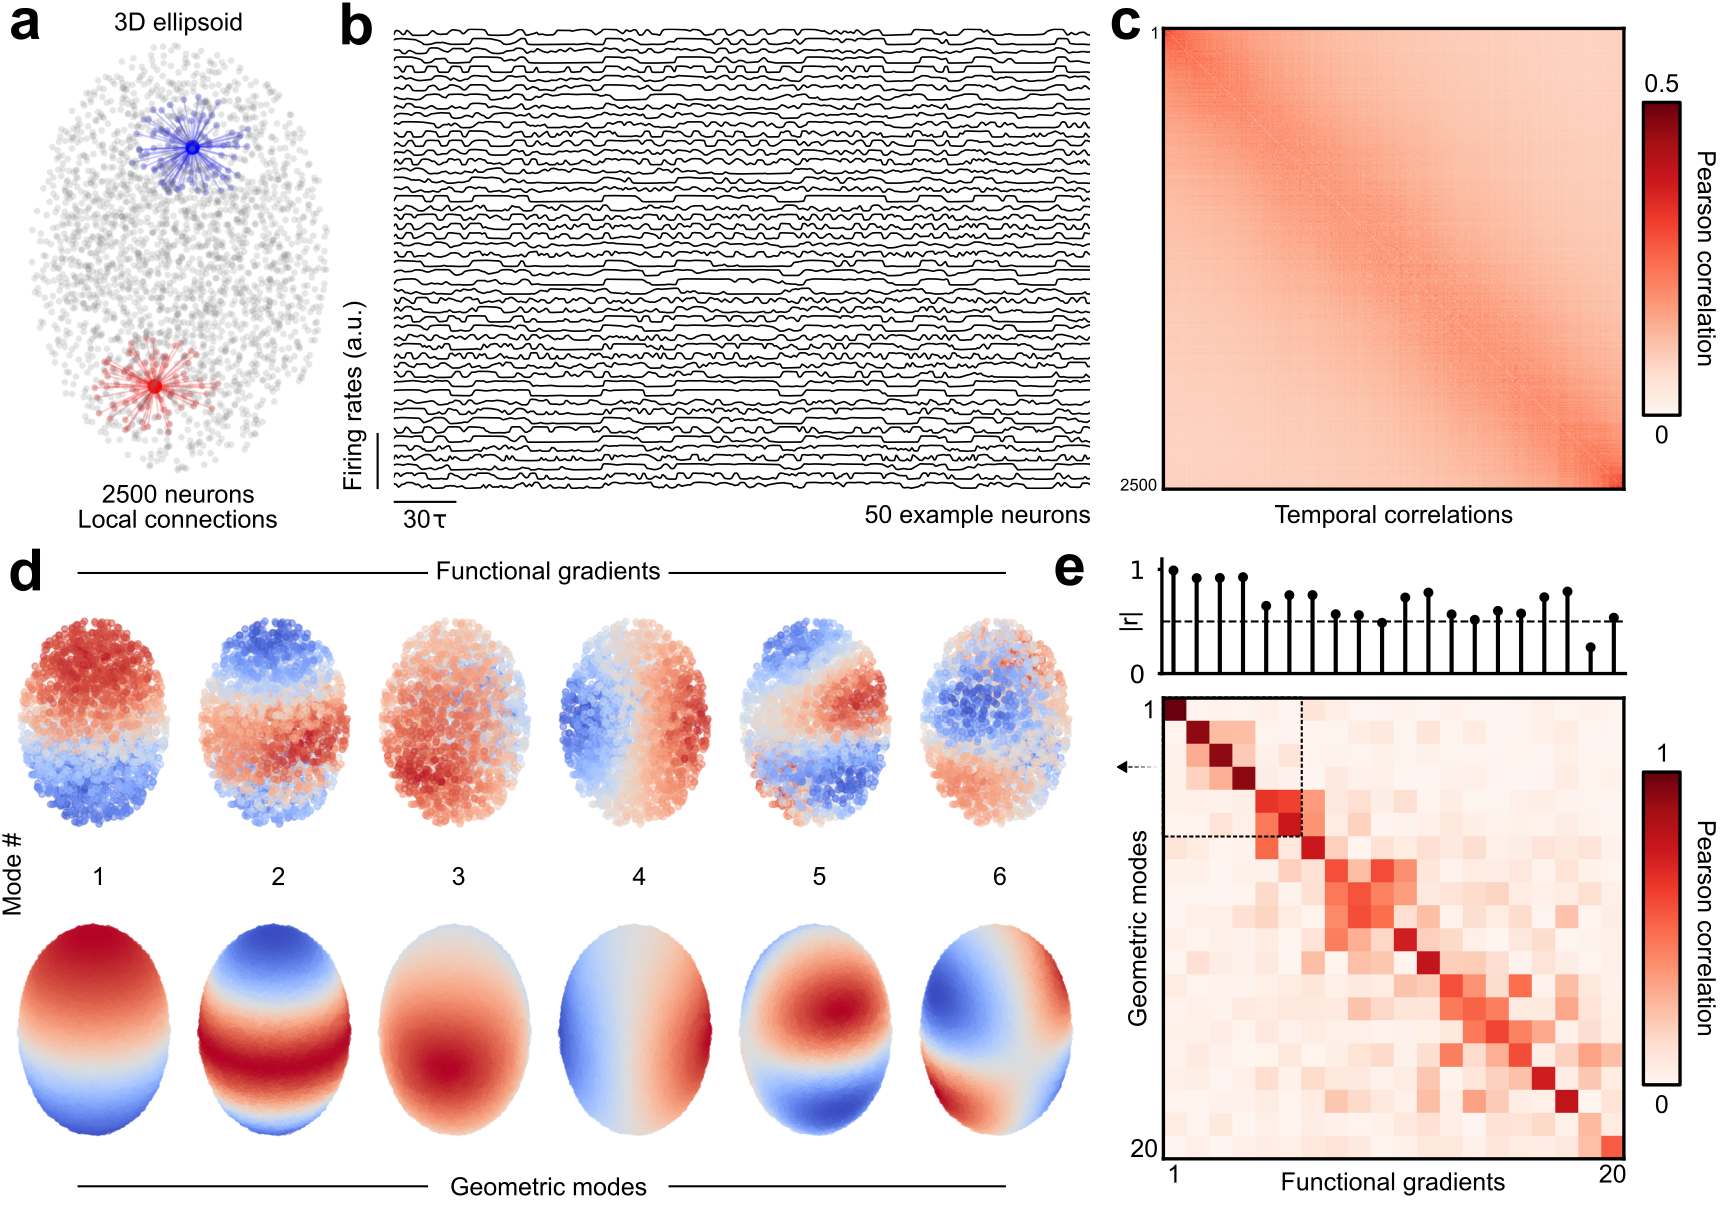
\includegraphics[width=0.95\textwidth]{Figures/figure1.png}
    \caption{}
    \label{fig1}
\end{figure*}

\section*{Discussion}


\section*{Methods}


\newpage

%\bibliographystyle{plain}
%\bibliography{reference.bib}

\section*{Acknowledgements}

We acknowledge Calcul Québec and Digital Research Alliance of Canada for their technical support and computing infrastructures.

\section*{Author contributions}

\section*{Competing interests}

The authors declare no competing interests.

\end{multicols}

\newpage

\section*{References}

Format de section temporaire: Voici quelques références importantes pour le projet.

\begin{enumerate}
    \item \fullcite{GarcaTrillos2019}
    \subitem Démonstration de la convergence entre l'opérateur Laplacien sur un graphe dans une variété de dimension $m$ et l'opérateur de Laplace-Beltrami dans la limite $N\to\infty$ et $h\to0$. Le voisinage de chacun des $N$ noeuds est contenu dans une sphère de rayon $h$.
\end{enumerate}



\newpage

\section*{Supplementary Material}


\end{document}